\documentclass[11pt]{article}
\usepackage[utf8]{inputenc}

\title{Recipe Recommendations}
\author{Easton Potokar}
\date{March 2020}

\usepackage{graphicx}
\usepackage{hyperref}
\usepackage{natbib}
\usepackage{amsmath}
\usepackage{xcolor}

\newcommand\todo[1]{\textcolor{red}{TODO: #1 \\}}
% \renewcommand\todo[1]{}

\newcommand*\textfrac[2]{
  \frac{\text{#1}}{\text{#2}}
}

\begin{document}

\maketitle

\begin{abstract}
    We seek to explore making a personalized recipe recommendation system based on ingredients, tags, and past user reviews. We analyze both the accuracy of the recommendations as well as the temporal complexity of making them. We find that we can make very accurate recommendations to satisfy what any cravings people may have and those didn't know they even had.
\end{abstract}

\section{Problem Statement and Motivation}
Machine Learning algorithms that make recommendations to users are becoming more and more common and are seen all over the internet for movies, friends, web searches, etc. A less common application is that of recipe suggestions. Is it possible to find a perfect recipe for someone given their past preferences of foods? Or a recommendation based on what their current cravings and pantry look like? 

\todo{More research on what's been already done.}

\section{Data}
Our data was gathered from \cite{data}, whose dataset can be found at \href{https://www.kaggle.com/shuyangli94/food-com-recipes-and-user-interactions}{here}. The data consists of more than 180 thousand recipes (made up of their ingredients, calorie level, and various tags describing them), and 700 thousand user reviews all scraped from Food.com ranging from 0 to 5 stars. The original authors of the data used various natural language processing techniques to parse the recipes into about 8 thousand unique ingredients, around 500 unique tags, and a calorie level that is a 0, 1, or 2 denoting low-calorie to high-calorie recipes.

The data appears to be very reliable, having been scraped directly from Food.com with the scraper being publicly available on github \cite{data_scraper}. Furthermore, it was used in a published research article, so one would hope everything was done ethically and correctly. The dataset is plenty large enough to give use meaningful answers to our questions and should be able to make a fairly robust recommendation system.

\section{Ethical Ramifications}
As with all recommendation systems, we must be careful what sort of bias we program into our algorithms. It would be very easily to heavily weight the algorithms to favor low-calorie recipes (healthier options) in an effort to push the public towards eating healthier. While this would likely be well intentioned, in a way it is removing one's freedom of options, and is manipulating user's behaviors. Many similar biases must also be carefully considered, whether it be toward a certain ingredient/brand (company sponsorship), a certain ethnic preference (potentially racist), etc.

\section{Methods}

We first put the data in a format useful for our algorithms. For our recipes, we make each recipe a vector, with a 1 in the $i$th entry denoting it having the $i$th ingredient or tag, and a 0 that it doesn't have it. We make the last entry that of calorie level. We format our user data in a similar way, only with the actual rating (from 0-5) of the $i$th recipe being in the $i$th entry.

However, this is a far from perfect solution. Note that the importance of a recipe having salt will be just as important as a recipe having jasmine or a jalapeno pepper. Commonly used in document classification, we use "TF-IDF" to help with this problem. In our case we change each entry using the conversion (where item means either ingredient/tag):

$$\textfrac{\# of $i$th item}{Total \# of items in Recipe} * \log \Big( \textfrac{Total \# of Recipes}{\# of Recipes with $i$th item} \Big)$$

We perform the same transformation on the user dataset, replacing item with rating, and recipes with users. Throughout this document we analyze our data in both forms in order to visualize which data helps the algorithms perform the best. (Spoiler: It's usually TF-IDF)

\subsection{Recommendation based on Recipe}
We first begin by reducing the dimensions of our data using PCA. After transforming the basis, we want to the keep the components that explain the majority of the variance in the data. These variances can be seen in Figure \ref{fig:pca}. We noted that for both, 100 components should be more than enough, with 20-40 likely being close to enough.
\begin{figure}[t]
\centering
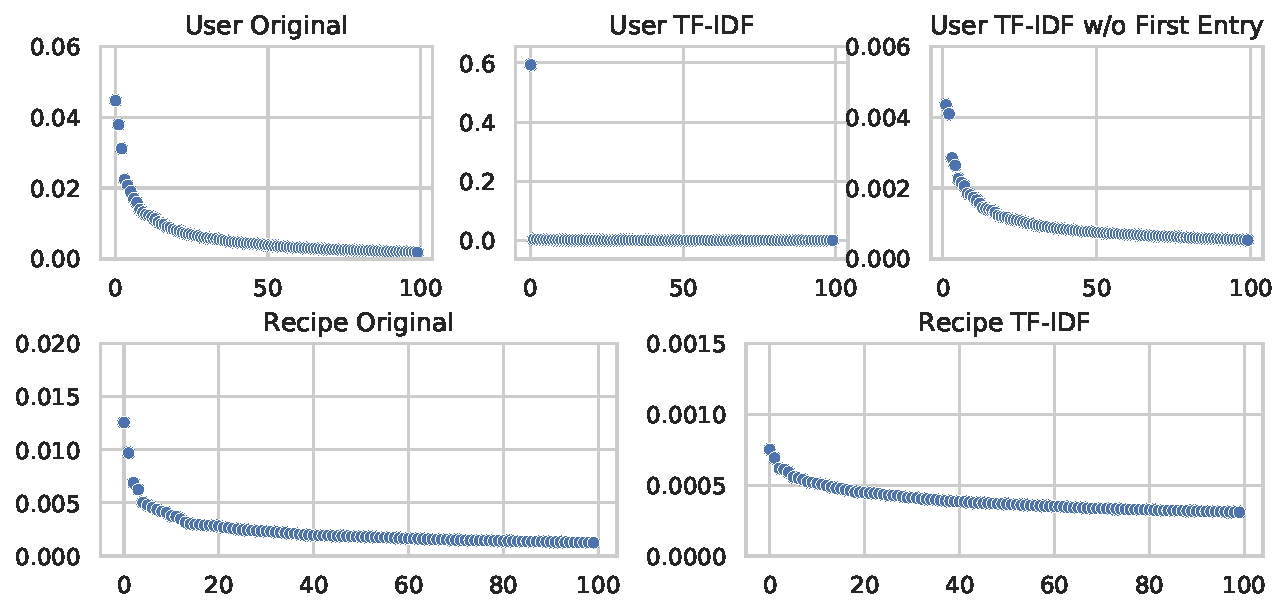
\includegraphics[width=1\textwidth]{figs/pca.pdf}
\caption{PCA Analysis of both Original and TF-IDF Recipe data}
\label{fig:pca}
\end{figure}

We next ran a Nearest Neighbor search to find the recipe that is the most similar, using KFold cross validation with K=7. We tried it with both the 2-norm and the cosine metric that will compute the "angle" between entries and timed each iteration of neighbor finding (what would need to be done on the fly) to see which combination is the most effective. We rated the results by the number of tags and ingredients the resulting recipe shared with the input recipe. The results are in Figures \ref{fig:recipe_nn_scores} and \ref{fig:recipe_nn_times}.

\begin{figure}[t]
\centering
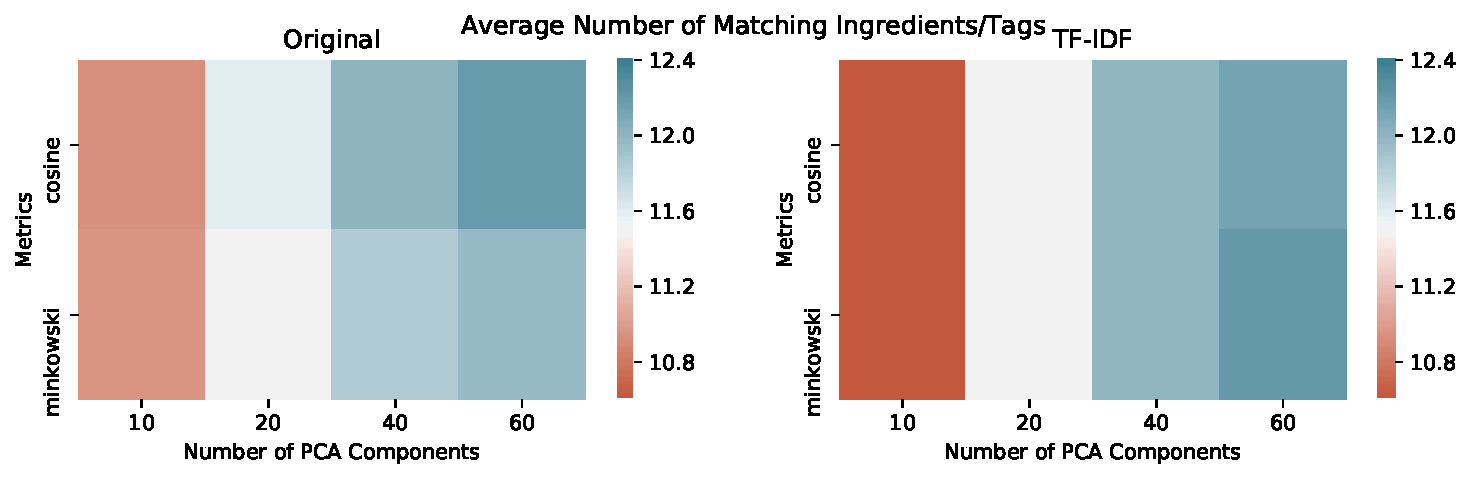
\includegraphics[width=1\textwidth]{figs/recipeNN_scores.pdf}
\caption{Results of Nearest Neighbor (scores)}
\label{fig:recipe_nn_scores}
\end{figure}

\begin{figure}[t]
\centering
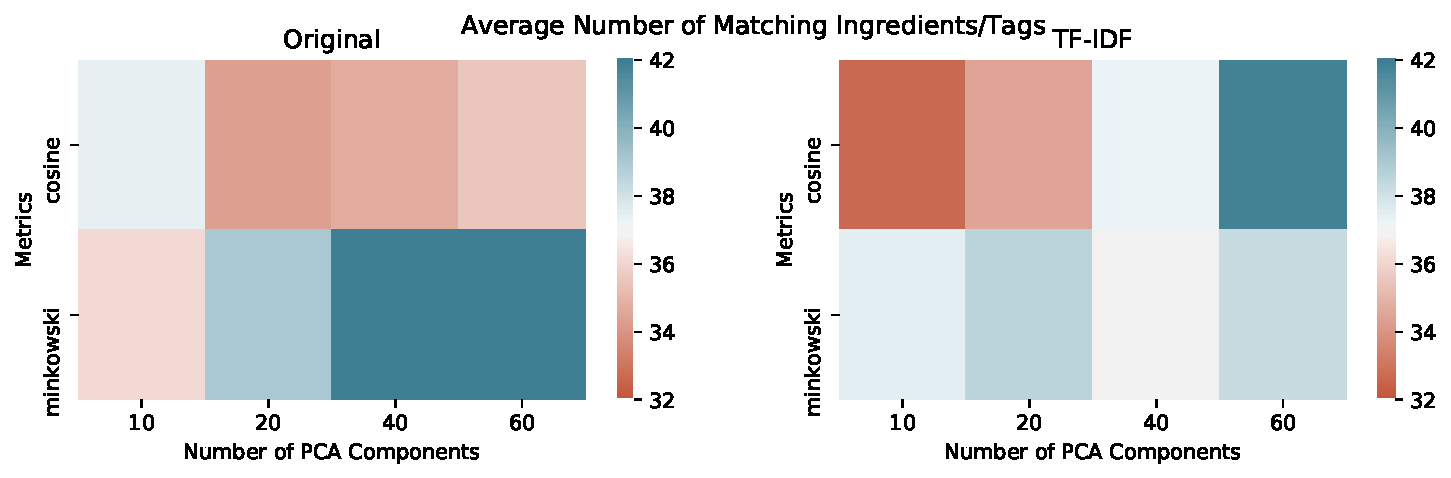
\includegraphics[width=1\textwidth]{figs/recipeNN_times.pdf}
\caption{Results of Nearest Neighbor (times)}
\label{fig:recipe_nn_times}
\end{figure}

Notice that the cosine metric was consistently faster (likely due to their being less operations to compute), while as far as accuracy, the metrics were a wash, as was the difference between TF-IDF and the original data.

Next, to see if we can reduce this time, we see if we can cluster the data, so we can find the cluster our test recipe belongs in, and then find the nearest neighbor in that set. We run UMAP first to identify clusters, although it won't be usable in production due to being unable to aggregate data to it (can't find what cluster our data point is in). As before, we vary various parameters to find the best fit. Results in Figure \ref{fig:recipe_umap}

\begin{figure}[t]
\centering
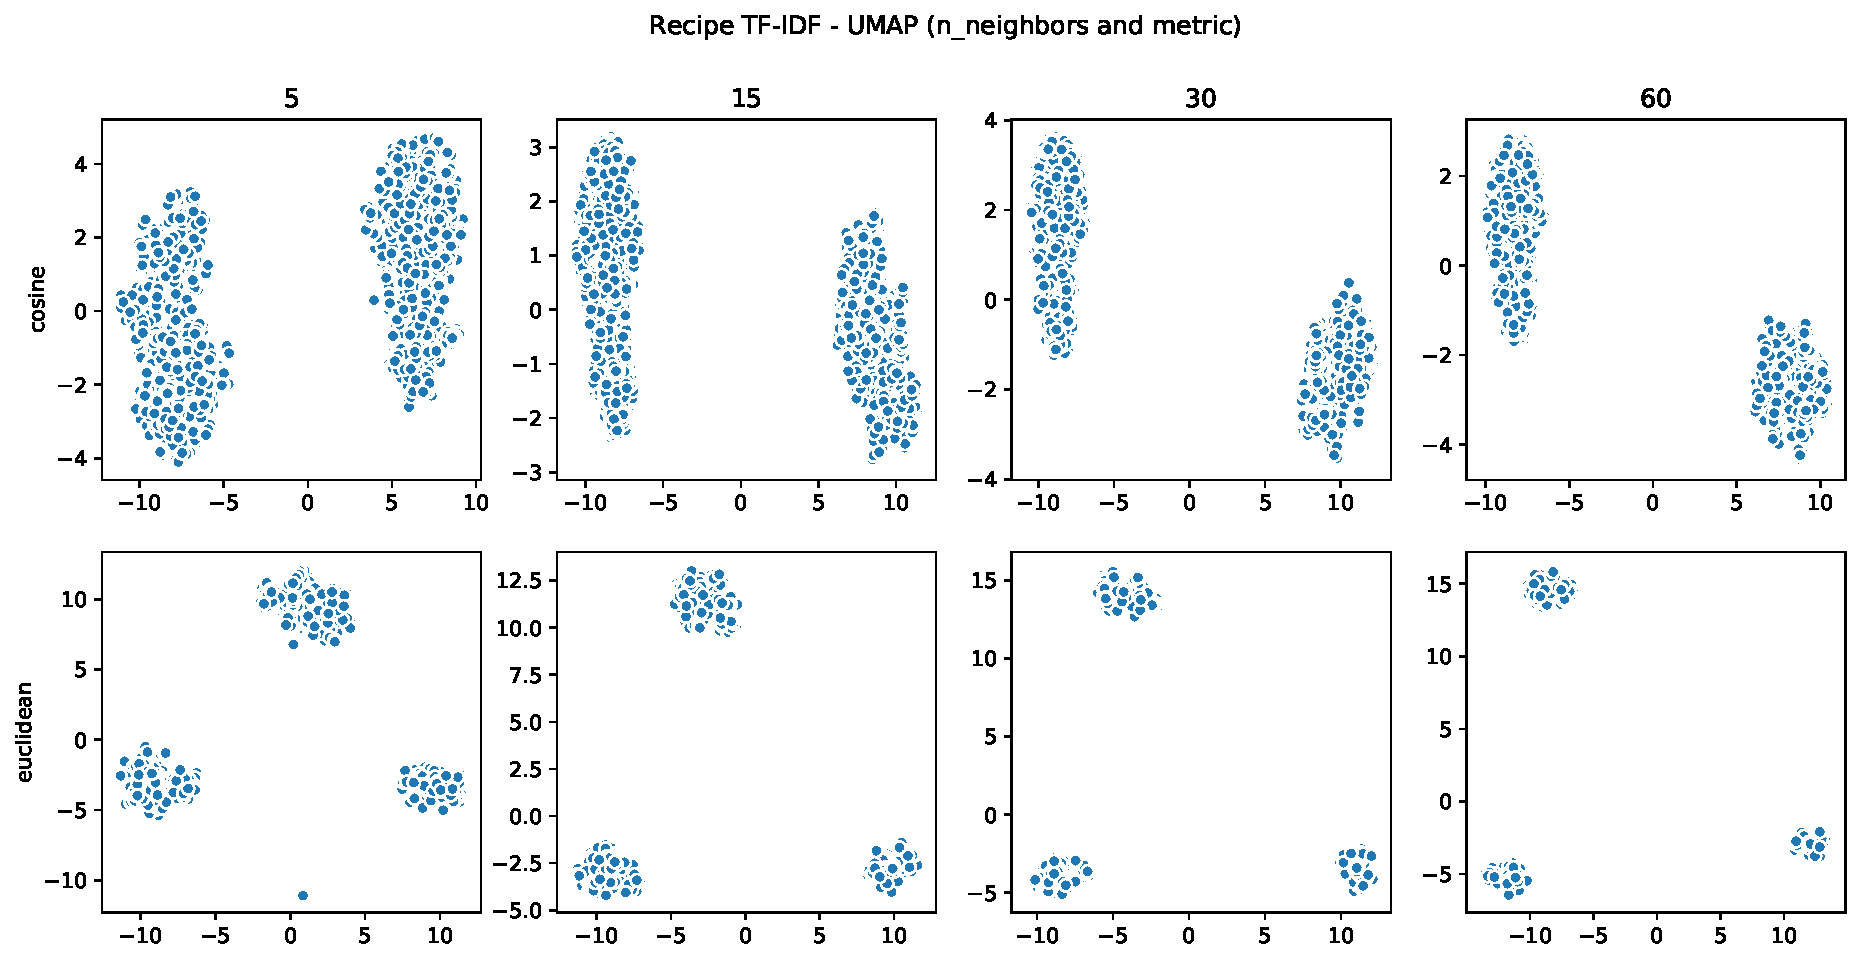
\includegraphics[width=1\textwidth]{figs/recipeUMAP_tfidf.pdf}
\caption{Results of UMAP on TF-IDF Recipe data}
\label{fig:recipe_umap}
\end{figure}

Note that UMAP with the euclidean norm identify 3 clusters very clearly!

\todo{Find defining features of UMAP clusters}
\todo{Try clustering algorithm that lets you test cluster of new data, see if using it with NN hinders results}
\subsection{Recommendation based on User}
Using the above results, we'll further cluster our user data to identify recipes that a user may enjoy.

We attempted using UMAP to identify clusters, but it performed very poorly.

\todo{Cluster User Data using Min-Cut, HMM, New Algorithm?}
\todo{NN User Data (try varying number of nearest neighbors)}
\todo{After clustering/NN, experiment with most common, closest, etc rated recipes in user group}
\todo{Weighted NN using ratings of single user? (Could be used as new algorithm)}

\section{Results}

\section{Analysis}

\section{Conclusion}

\bibliographystyle{plain}
\bibliography{references}
\end{document}
